\section{Procedimentos metodológicos}
\label{sec:metodo}

Este capítulo descreve, na ordem em que são executados, os procedimentos que
transformam os microdados públicos da Pesquisa Nacional por Amostra de
Domicílios Contínua (PNADC) em um painel de transições de trabalho e, a partir
dele, em estimativas de gradiente de exposição ocupacional à inteligência
artificial. A descrição segue exatamente o que é implementado: cada regra de
seleção, cada definição de desfecho e cada especificação apresentada aqui
corresponde a uma etapa concreta do procedimento, e as quantidades reportadas
são as efetivamente obtidas. O desenho apresentado é deliberadamente enxuto ---
um único cenário de estimação, sem bateria de sensibilidades ---, e a agenda de
robustez que ele deixa em aberto está organizada no Capítulo~\ref{sec:melhorias}.

\subsection{Roteiro de execução e reprodutibilidade}
\label{sec:roteiro}

O procedimento é executado como uma cadeia de sete etapas numeradas, cada uma
com um script próprio, uma saída própria e um registro próprio de execução. A
numeração não é decorativa: cada etapa só pode rodar depois que a anterior
gravou seu artefato, e nenhuma etapa recalcula o que a anterior já produziu. O
Quadro~\ref{qua:etapas} apresenta a correspondência completa entre a descrição
metodológica das seções seguintes e o código que a implementa.

\begin{quadro}[htbp]
  \caption{Etapas do procedimento, scripts correspondentes e artefatos produzidos}
  \label{qua:etapas}
  \centering
  \espacosimples\idpcorpodez
  \begin{tabular}{@{}p{0.9cm}p{3.9cm}p{4.5cm}p{5.0cm}@{}}
    \toprule
    \textbf{Etapa} & \textbf{Script executado} & \textbf{O que faz} & \textbf{Artefato produzido} \\
    \midrule
    00 & \texttt{00\_ambiente.py} \newline \texttt{src/setup.py}
       & Registra versões de pacotes e confirma o acesso ao repositório de dados.
       & Registro de ambiente em \texttt{logs/} \\
    \addlinespace[2pt]
    01 & \texttt{01\_dicionarios.py} \newline \texttt{src/dictionaries.py}
       & Lê o dicionário oficial da pesquisa e traduz as categorias por rótulo,
         sem código digitado à mão.
       & \texttt{dicionario\_br\_ibge\_pnadc} \newline \texttt{dicionarios\_verificados.json} \\
    \addlinespace[2pt]
    02 & \texttt{02\_insumos.py} \newline \texttt{src/insumos.py}
       & Lê a medida de exposição e a de teletrabalhabilidade, audita a estrutura
         ocupacional brasileira, constrói a ponte ocupacional e agrega a
         exposição por código (Seção~\ref{sec:exposicao}).
       & \texttt{exposicao\_cod.parquet} \newline \texttt{auditoria\_cod\_isco.json} \\
    \addlinespace[2pt]
    03 & \texttt{03\_cobertura\_pnadc.py} \newline \texttt{src/pnadc/pareamento.py}
       & Verifica quais trimestres estão disponíveis na fonte e delimita a janela
         efetivamente utilizável.
       & \texttt{pnadc\_cobertura.parquet} \\
    \addlinespace[2pt]
    04 & \texttt{04\_painel\_pnadc.py} \newline \texttt{src/pnadc/pareamento.py}
       & Executa a autojunção entre trimestres consecutivos no ambiente remoto,
         aplica as regras de identidade da Seção~\ref{sec:par}, calcula os
         desfechos e desce apenas células agregadas.
       & \texttt{pnadc\_transicoes.parquet} \newline \texttt{pnadc\_taxa\_pareamento.parquet} \\
    \addlinespace[2pt]
    05 & \texttt{05\_estimacao.py} \newline \texttt{src/estimacao.py}
       & Estima os sete modelos de probabilidade linear da
         equação~\eqref{eq:principal} e calcula a matriz de mobilidade com
         reamostragem por unidade primária.
       & Coeficientes, covariâncias e metadados em \texttt{output/modelos/} \\
    \addlinespace[2pt]
    06 & \texttt{06\_tabelas\_figuras.py} \newline \texttt{src/resultados.py}
       & Consolida os modelos salvos em tabelas e figuras. Não reestima nada.
       & \texttt{output/tabelas/}, \texttt{output/figuras/} e o relatório de resultados \\
    \bottomrule
  \end{tabular}
  \fonte{Elaboração própria (2026).}
  \nota{Os scripts ficam em \texttt{scripts/} e os módulos em \texttt{src/}. A
        cadeia inteira é disparada por \texttt{executa\_tudo.py}; as etapas 05 e
        06 podem ser refeitas isoladamente a partir do painel já construído.}
\end{quadro}

Três garantias de reprodutibilidade acompanham essa cadeia e são parte do
método, não detalhe de implementação. A primeira é a restrição de dados:
microdados individuais não são materializados localmente em nenhuma etapa, e a
rotina de consulta recusa qualquer consulta sem agregação. A segunda é o
registro de execução: cada etapa grava início, fim, situação e o resultado
retornado, de modo que uma etapa interrompida não é confundida com uma etapa
concluída. A terceira é o rastro criptográfico: cada modelo estimado grava, ao
lado dos coeficientes, a fórmula executada, o nível de agrupamento, a variável
de ponderação, o número de grupos e a impressão \textit{SHA-256} do arquivo de
dados que efetivamente entrou na estimação, junto com uma cópia congelada do
script que rodou.

\subsection{Fonte e unidade de observação}

A fonte é a PNADC trimestral do Instituto Brasileiro de Geografia e Estatística
(IBGE), acessada por meio do repositório público Base dos Dados
\parencite{basedosdados_pnadc}. A janela considerada vai do primeiro trimestre
de 2019 ao quarto trimestre de 2025, o que corresponde a vinte e sete
trimestres elegíveis como trimestre de origem, de 2019T1 a 2025T3.

A PNADC é uma pesquisa domiciliar de painel rotativo: cada domicílio
selecionado é entrevistado em cinco visitas trimestrais consecutivas e depois
substituído. Essa estrutura é o que torna possível observar o mesmo indivíduo em
dois trimestres consecutivos e, portanto, medir transições em vez de estoques.

A unidade de observação deste trabalho é o \textbf{par pessoa-trimestre}: a
entrevista de origem no trimestre $t$ ligada à entrevista do mesmo indivíduo no
trimestre $t+1$. Todas as covariáveis e a exposição pertencem à \emph{origem} do
par; os desfechos são definidos pela comparação entre origem e destino.

Uma restrição operacional foi imposta desde o início e condiciona todo o
procedimento: \textbf{microdados individuais não são materializados
localmente}. O pareamento entre entrevistas consecutivas é executado no próprio
ambiente de consulta remoto do repositório, e o que é trazido para a análise são
\emph{células agregadas} por trimestre, unidade da federação (UF), unidade
primária de amostragem (UPA), ocupação de origem, ocupação de destino e o
conjunto completo de covariáveis do modelo. Cada célula carrega a contagem de
pessoas $n$, a soma dos pesos amostrais e a soma dos quadrados dos pesos.

Essa agregação não é uma aproximação. Como todas as variáveis explicativas e
todos os desfechos são constantes dentro de cada célula por construção --- a
célula é definida justamente pela combinação exata dessas variáveis ---, a
estimação ponderada em células reproduz exatamente a estimação ponderada em
indivíduos. Formalmente, se $\mathcal{C}$ é uma célula e $y_i = y_{\mathcal{C}}$
e $x_i = x_{\mathcal{C}}$ para todo $i \in \mathcal{C}$, então

\begin{equation}
  \sum_{i \in \mathcal{C}} w_i \, x_i x_i' = \left( \sum_{i \in \mathcal{C}} w_i \right) x_{\mathcal{C}} x_{\mathcal{C}}',
  \qquad
  \sum_{i \in \mathcal{C}} w_i \, x_i y_i = \left( \sum_{i \in \mathcal{C}} w_i \right) x_{\mathcal{C}} y_{\mathcal{C}},
  \label{eq:agregacao}
\end{equation}

de modo que os coeficientes de mínimos quadrados ponderados e os escores usados
na inferência agrupada são idênticos aos da estimação individual, desde que o
nível de agrupamento seja mais grosso que a célula --- o que é o caso, já que a
UPA contém células inteiras.

\subsection{Construção do par pessoa-trimestre}
\label{sec:par}

Não existe identificador longitudinal individual validado na PNADC pública. O
par é construído por identidade reconstruída, exigindo simultaneamente todas as
condições a seguir entre a entrevista de origem $a$ e a entrevista candidata a
destino $b$:

\begin{enumerate}[label=\alph*)]
  \item mesma UPA, mesmo domicílio e mesmo número de ordem do indivíduo na
        família;
  \item trimestre imediatamente seguinte e visita imediatamente seguinte, isto
        é, $t_b = t_a + 1$ e $v_b = v_a + 1$;
  \item mesmo sexo declarado;
  \item mesmo dia e mesmo mês de nascimento, com dia entre 1 e 31 e mês entre 1
        e 12;
  \item ano de nascimento diferindo em no máximo um ano, o que acomoda erro de
        registro sem admitir troca de pessoa;
  \item idade que avança zero ou um ano, isto é, $\text{idade}_b \in
        \{\text{idade}_a, \text{idade}_a + 1\}$;
  \item chave de identificação não duplicada dentro do trimestre, dos dois
        lados do par.
\end{enumerate}

A condição (g) é conservadora por decisão: quando a combinação de UPA,
domicílio e número de ordem aparece mais de uma vez no mesmo trimestre, o
registro não é pareado em nenhuma direção, em vez de ser resolvido por
critério arbitrário. A condição (b) implica que a quinta visita nunca entra como
origem, pois não há visita seguinte, e que o último trimestre disponível não
entra no denominador de atrito.

A qualidade do pareamento é monitorada trimestre a trimestre. A taxa ponderada
de pareamento varia entre 0,747 e 0,847 ao longo dos vinte e sete trimestres, e
os valores mais baixos concentram-se em 2020 e 2021, período em que a coleta da
PNADC foi feita majoritariamente por telefone em razão da pandemia
\parencite{ibge2022tratamento}. A Figura~\ref{fig:pareamento} apresenta a série.

\begin{figure}[htb]
  \caption{Taxa ponderada de pareamento, por trimestre de origem}
  \label{fig:pareamento}
  \centering
  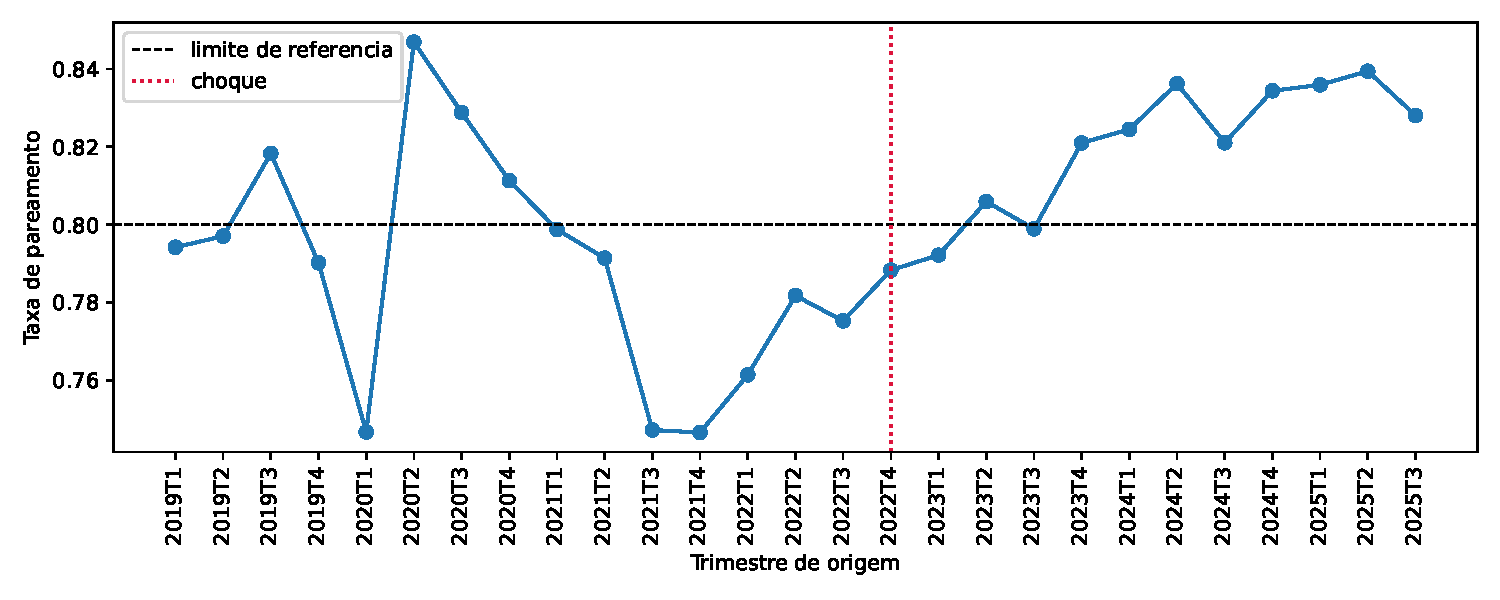
\includegraphics[width=0.92\textwidth]{figuras/fig_taxa_pareamento.pdf}
  \fonte{Elaboração própria a partir da PNADC/IBGE (2019T1--2025T3).}
  \nota{A linha de referência é 0,80. Os trimestres abaixo dela concentram-se no
        período de coleta atípica de 2020--2021.}
\end{figure}

\subsection{Filtragem da amostra}
\label{sec:filtragem}

A amostra analítica é obtida por uma sequência de cortes, todos justificados por
uma regra de desenho e nenhum por conveniência de resultado. A
Figura~\ref{fig:funil} apresenta o passo a passo com as quantidades efetivas em
cada etapa, medidas em pessoas-transições, isto é, na contagem de indivíduos
subjacente às células.

\begin{figure}[htbp]
  \caption{Passo a passo da filtragem dos dados, da PNADC aos domínios de estimação}
  \label{fig:funil}
  \centering
  \espacosimples
  \begin{tikzpicture}[
      font=\fontsize{8}{9.6}\selectfont,
      caixa/.style={draw, rounded corners=2pt, align=left, inner sep=4pt,
                    text width=6.5cm, fill=black!3},
      corte/.style={draw=black!45, dashed, rounded corners=2pt, align=left,
                    inner sep=4pt, text width=6.7cm, fill=white},
      seta/.style={-{Stealth[length=4pt]}, thick, black!65},
      lig/.style={-{Stealth[length=3pt]}, black!45}
    ]
    \node[caixa] (a) {\textbf{A. PNAD Contínua trimestral}\\
      2019T1 a 2025T4, painel rotativo de cinco visitas};
    \node[caixa, below=8mm of a] (b) {\textbf{B. Origens elegíveis}\\
      \textbf{4.017.289} pessoas-transições \hfill 27 trimestres};
    \node[caixa, below=8mm of b] (c) {\textbf{C. Exposição atribuída à origem}\\
      \textbf{3.963.359} \hfill 98,7\% de B \; -- \; 413 ocupações};
    \node[caixa, below=8mm of c] (d) {\textbf{D. Par encontrado}\\
      \textbf{3.178.582} \hfill 80,2\% de C};
    \node[caixa, below=8mm of d] (e) {\textbf{E. Destino ocupado}\\
      \textbf{2.882.225} \hfill 90,7\% de D};
    \node[caixa, below=8mm of e, fill=black!8] (f) {\textbf{F. Domínio de mobilidade}\\
      \textbf{2.879.139} \hfill 99,9\% de E};
    \node[caixa, below=8mm of f] (g) {\textbf{G. Domínio de formalidade}\\
      \textbf{1.677.310} \hfill 52,8\% de D};

    \foreach \x/\y in {a/b, b/c, c/d, d/e, e/f, f/g} {\draw[seta] (\x) -- (\y);}

    \node[corte, right=6mm of a.east, anchor=west, yshift=-4mm] (ra)
      {Pessoa ocupada, 18 a 65 anos, visitas 1 a 4, trimestre com trimestre
       seguinte disponível};
    \node[corte, right=6mm of b.east, anchor=west, yshift=-4mm] (rb)
      {AIOE e teletrabalhabilidade disponíveis para a ocupação de origem;
       militares e ocupações sem correspondência ficam de fora};
    \node[corte, right=6mm of c.east, anchor=west, yshift=-4mm] (rc)
      {Identidade reconstruída e validada: domicílio, ordem, visita seguinte,
       sexo, data de nascimento, idade coerente, chave não duplicada};
    \node[corte, right=6mm of d.east, anchor=west, yshift=-4mm] (rd)
      {Condição de ocupação no destino igual a ocupado};
    \node[corte, right=6mm of e.east, anchor=west, yshift=-4mm] (re)
      {Código ocupacional e AIOE observados na origem \emph{e} no destino};
    \node[corte, right=6mm of f.east, anchor=west, yshift=-4mm] (rf)
      {Ramo próprio, a partir de D: origem formal e destino observado};

    \foreach \x/\y in {a/ra, b/rb, c/rc, d/rd, e/re, f/rf}
      {\draw[lig] (\x.east) -- (\y.west);}
  \end{tikzpicture}
  \fonte{Elaboração própria a partir da PNADC/IBGE.}
  \nota{As quantidades são pessoas-transições, não pessoas únicas: o mesmo
        indivíduo contribui com até quatro pares. Cada desfecho usa o domínio em
        que está definido: o teste de atrito usa todas as origens de C; a saída
        do emprego usa D; a mudança de ocupação usa E; as margens direcionais
        usam F; e a informalização usa G, que é um ramo lateral de D e não uma
        continuação de F.}
\end{figure}

Duas observações sobre a filtragem merecem destaque, porque afetam a leitura
dos resultados. Primeira: cada desfecho tem seu próprio domínio, e ausência
nunca é convertida em zero --- um destino não observado não é ``não mudou de
ocupação'', é simplesmente indefinido. Segunda: as quantidades são
pessoas-transições e não pessoas únicas, de modo que um mesmo indivíduo pode
contribuir com até quatro pares ao longo do painel, e os pesos amostrais somados
não são contagens de indivíduos independentes.

\subsection{Medida de exposição à inteligência artificial}
\label{sec:exposicao}

O tratamento é o \textit{Artificial Intelligence Occupational Exposure} (AIOE)
de \citeonline{felten2021}, publicado na classificação ocupacional americana
\textit{Standard Occupational Classification} de 2010 (SOC2010). A PNADC
classifica ocupação segundo a Classificação de Ocupações para Pesquisas
Domiciliares (COD), adaptação brasileira da \textit{International Standard
Classification of Occupations} de 2008 (ISCO-08). É necessária, portanto, uma
ponte em duas etapas: COD $\rightarrow$ ISCO-08 $\rightarrow$ SOC2010.

\subsubsection{Construção da ponte ocupacional}

A ponte é construída com resolução declarada elo a elo, e não por semelhança
numérica genérica:

\begin{enumerate}[label=\alph*)]
  \item grupos civis são comparados em quatro dígitos;
  \item o grupo 6 (agropecuária) é comparado em dois dígitos, porque o IBGE
        reagrupa esse bloco e a repartição fina seria arbitrária;
  \item entradas agregadas de três dígitos da correspondência oficial
        ISCO-SOC são incorporadas explicitamente;
  \item ocupações militares e o código 5168 não recebem exposição atribuída;
  \item entre os códigos SOC associados a um mesmo código COD, o peso é
        uniforme.
\end{enumerate}

A hipótese (e) é uma hipótese de construção declarada, não uma probabilidade
oficial de correspondência. Dos 434 códigos COD de quatro dígitos da estrutura
oficial, 427 recebem ao menos um elo, totalizando 1.148 elos, e o número máximo
de códigos SOC associados a um único COD é 37.

\subsubsection{Agregação da exposição para o código ocupacional}

Seja $S(c)$ o conjunto de códigos SOC ligados ao código ocupacional $c$, com
pesos $\omega_{cs} = 1/|S(c)|$. A exposição do código $c$ é a média ponderada

\begin{equation}
  A_c \;=\; \frac{\displaystyle\sum_{s \in S(c)} \omega_{cs} \, A_s \, \mathbb{1}\{A_s \text{ observado}\}}
                 {\displaystyle\sum_{s \in S(c)} \omega_{cs} \, \mathbb{1}\{A_s \text{ observado}\}},
  \label{eq:agregacao_exposicao}
\end{equation}

de modo que elos sem valor observado são \emph{ignorados} no cálculo, e não
tratados como zero --- tratá-los como zero introduziria atenuação mecânica
proporcional à incompletude da ponte. O mesmo procedimento é aplicado ao índice
de teletrabalhabilidade de \citeonline{dingel2020}, usado como controle.

A cobertura resultante é alta: 416 códigos COD recebem exposição e 413 recebem
também teletrabalhabilidade, sendo esses 413 os que entram na estimação. A
fração do peso amostral sem AIOE atribuído na origem é de 1,08\%, bem abaixo do
limite de 15\% fixado como critério de aceitação antes da estimação.

\subsubsection{Escala e padronização}

O AIOE é padronizado \emph{entre ocupações}, e não entre trabalhadores. Entre os
416 códigos COD com exposição, a média é 0,0053 e o desvio-padrão é
$\sigma_A = 0{,}9445$, praticamente unitário. Um coeficiente estimado ``por
unidade de AIOE'' lê-se, portanto, como ``por desvio-padrão de exposição entre
ocupações'', e é assim que todo coeficiente é reportado no
Capítulo~\ref{sec:resultados}. Ponderando por trabalhador, a média cai para
$-0{,}221$ e o desvio-padrão sobe para $0{,}981$: o emprego brasileiro
concentra-se em ocupações de exposição abaixo da média entre ocupações. A
Figura~\ref{fig:distribuicao} mostra a distribuição.

\begin{figure}[htb]
  \caption{Distribuição do AIOE entre códigos ocupacionais}
  \label{fig:distribuicao}
  \centering
  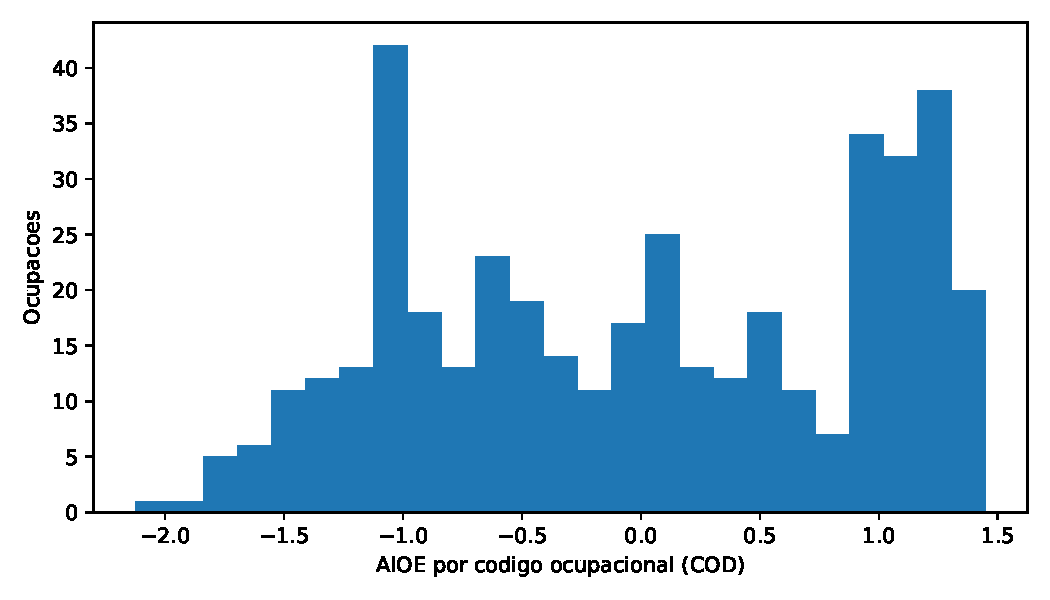
\includegraphics[width=0.85\textwidth]{figuras/fig_distribuicao_aioe.pdf}
  \fonte{Elaboração própria a partir de \citeonline{felten2021} e da PNADC/IBGE.}
\end{figure}

Uma segunda advertência de leitura decorre da escala e deve acompanhar todo
coeficiente reportado: AIOE menor significa \emph{menos exposição}, não emprego
pior, salário menor ou posição inferior na hierarquia ocupacional.

\subsubsection{Correlação com teletrabalhabilidade}

A correlação entre AIOE e teletrabalhabilidade entre códigos ocupacionais é de
$0{,}702$. Ocupações expostas à inteligência artificial são, em larga medida, as
mesmas ocupações que podem ser exercidas remotamente. Como o período analisado
contém a reorganização do trabalho remoto no pós-pandemia, omitir a
teletrabalhabilidade faria o coeficiente de exposição absorver essa
reorganização. Por isso o índice de teletrabalhabilidade entra na especificação
interagido com o indicador de período, exatamente na mesma forma funcional que o
tratamento.

\subsection{Definição dos desfechos}

São sete desfechos, organizados em três famílias e apresentados no
Quadro~\ref{qua:desfechos}. Seja $c(i)$ o código ocupacional de origem do par
$i$, $c'(i)$ o de destino, e $A_c$ a exposição da ocupação $c$ dada pela
equação~\eqref{eq:agregacao_exposicao}.

\begin{quadro}[htbp]
  \caption{Desfechos, definição formal e domínio de estimação}
  \label{qua:desfechos}
  \centering
  \espacosimples\idpcorpodez
  \begin{tabular}{@{}p{3.5cm}p{6.3cm}p{4.9cm}@{}}
    \toprule
    \textbf{Desfecho} & \textbf{Definição} & \textbf{Domínio} \\
    \midrule
    \multicolumn{3}{@{}l}{\textit{(i) Continuidade e vínculo}} \\
    \addlinespace[2pt]
    Pareamento
      & $1$ se a entrevista seguinte foi encontrada
      & todas as origens elegíveis \\
    Saída do emprego
      & $1$ se o destino não está ocupado
      & pares \\
    Formal para informal
      & $1$ se a origem é formal e o destino está ocupado e é informal
      & pares com origem formal e destino observado \\
    \addlinespace[3pt]
    \multicolumn{3}{@{}l}{\textit{(ii) Mobilidade ocupacional}} \\
    \addlinespace[2pt]
    Muda de ocupação (2 dígitos)
      & $1$ se $c'(i) \neq c(i)$ nos dois primeiros dígitos
      & pares com destino ocupado e ambos os códigos observados \\
    Muda de ocupação (3 dígitos)
      & $1$ se $c'(i) \neq c(i)$ nos três primeiros dígitos
      & idem \\
    \addlinespace[3pt]
    \multicolumn{3}{@{}l}{\textit{(iii) Deslocamento no gradiente de exposição}} \\
    \addlinespace[2pt]
    Mobilidade descendente
      & $1$ se $A_{c'(i)} < A_{c(i)}$
      & pares com AIOE observado nos dois lados \\
    Mobilidade ascendente
      & $1$ se $A_{c'(i)} > A_{c(i)}$
      & idem \\
    \bottomrule
  \end{tabular}
  \fonte{Elaboração própria (2026).}
\end{quadro}

A classificação de formalidade segue o dicionário oficial da pesquisa e não
admite código digitado à mão: empregado com carteira assinada, militar e
estatutário são formais; empregado sem carteira e trabalhador familiar auxiliar
são informais; conta-própria e empregador são classificados como formais
\emph{apenas} quando declaram inscrição no Cadastro Nacional da Pessoa Jurídica
(CNPJ), e ficam indefinidos quando a declaração está ausente. A escolha de
deixar indefinido em vez de imputar informalidade é deliberada: a alternativa
introduziria correlação espúria entre informalidade medida e não resposta.

O desfecho de pareamento cumpre função distinta das demais. Ele não é um
resultado de interesse substantivo, e sim um \textbf{teste de atrito}: se a
exposição da ocupação de origem previsse quem desaparece do painel, todos os
demais desfechos, definidos apenas sobre pares completos, estariam contaminados
por seleção. A leitura correta é a de um teste de falseamento, em que não
rejeitar é o resultado desejável.

O par de margens direcionais --- mobilidade descendente e ascendente --- é
sempre lido em conjunto, e nunca isoladamente. Quem parte de exposição alta só
pode se deslocar para baixo no gradiente, e vice-versa; a assimetria de nível é
mecânica e é absorvida pelo efeito fixo de ocupação, de modo que o contraste
informativo é a diferença entre os períodos, não o nível de cada margem.

\subsection{Análise descritiva}

A descrição precede e condiciona a estimação, e cobre dois blocos.

\subsubsection{Médias ponderadas por período}

Para cada desfecho calcula-se a média ponderada pelo peso amostral da origem no
período pré e no período pós, no domínio próprio daquele desfecho. Esse bloco
fixa a ordem de grandeza: antes de qualquer efeito diferencial, ele mostra
quanta rotatividade existe em um trimestre normal do mercado de trabalho
brasileiro, e permite julgar se um coeficiente de fração de ponto percentual é
grande ou pequeno em relação à margem que pretende explicar.

\subsubsection{Matriz de mobilidade entre faixas de exposição}

Os códigos ocupacionais são divididos em cinco faixas de exposição, com cortes
nos quintis da distribuição do AIOE \emph{entre códigos ocupacionais}, e não
entre trabalhadores. A escolha é deliberada: quintis definidos entre pessoas
seriam redefinidos pela própria recomposição do emprego, contaminando a
comparação entre períodos com a mudança que se pretende medir. As faixas são
fixas e idênticas no pré e no pós.

Para cada faixa de origem $q$ e cada faixa de destino $r$, calcula-se a
probabilidade ponderada de transição em cada período,

\begin{equation}
  \widehat{P}^{\,p}_{qr} \;=\;
  \frac{\displaystyle\sum_{i \in \mathcal{P}_p} w_i \, \mathbb{1}\{q_i = q, \, r_i = r\}}
       {\displaystyle\sum_{i \in \mathcal{P}_p} w_i \, \mathbb{1}\{q_i = q\}},
  \qquad p \in \{\text{pré}, \text{pós}\},
  \label{eq:matriz}
\end{equation}

e o objeto de interesse é a diferença $\widehat{D}_{qr} = \widehat{P}^{\,
\text{pós}}_{qr} - \widehat{P}^{\,\text{pré}}_{qr}$.

A incerteza vem de uma \textbf{reamostragem por unidade primária de amostragem}.
Em cada uma das 199 réplicas, sorteiam-se UPAs com reposição por um esquema
multinomial e a UPA inteira entra na réplica com suas observações pré e pós
conjuntas. Sortear o cluster inteiro, e não separadamente por período, preserva
tanto a correlação dentro da UPA quanto a dependência entre os dois períodos.

O teste de igualdade das matrizes pré e pós é um teste de Wald construído sobre
a matriz de covariância $\widehat{\Sigma}$ das réplicas. Empilhando as $25$
diferenças no vetor $\widehat{d}$,

\begin{equation}
  W \;=\; \widehat{d}^{\,\prime} \, \widehat{\Sigma}^{+} \, \widehat{d}
  \;\;\sim\;\; \chi^2_{\,\mathrm{posto}(\widehat{\Sigma})},
  \label{eq:wald}
\end{equation}

com $\widehat{\Sigma}^{+}$ denotando a pseudo-inversa de Moore-Penrose. O uso da
pseudo-inversa e dos graus de liberdade iguais ao posto é necessário porque as
linhas da matriz de transição somam um, o que torna $\widehat{\Sigma}$
singular por construção.

\subsection{Especificação econométrica}
\label{sec:espec}

\subsubsection{Desenho}

O desenho é de \textbf{diferenças em diferenças com tratamento contínuo}. Não há
grupo tratado e grupo de controle: há um marco temporal único e nacional --- o
lançamento público do ChatGPT, em 30 de novembro de 2022 --- e uma intensidade
de tratamento que varia entre ocupações, dada pela exposição da ocupação de
origem. O parâmetro de interesse é o \emph{gradiente} de resposta por
desvio-padrão de exposição, e não o efeito de um tratamento binário
\parencite{callaway2024}.

O indicador de período é definido no trimestre do marco:

\begin{equation}
  \text{Pós}_t =
  \begin{cases}
    1, & t \geq 2022\text{T}4, \\
    0, & t \leq 2022\text{T}3.
  \end{cases}
  \label{eq:pos}
\end{equation}

São, portanto, quinze trimestres de origem no período pré, de 2019T1 a 2022T3, e
doze no pós, de 2022T4 a 2025T3. O trimestre do marco é classificado como pós
por convenção declarada antes da estimação; ele contém dois meses anteriores ao
lançamento, e essa ambiguidade é registrada como limite conhecido, não corrigida
por exclusão.

\subsubsection{Equação estimada}

Para um par $i$ com ocupação de origem $c$, unidade da federação $u$ e trimestre
de origem $t$, estima-se

\begin{equation}
\begin{split}
  y_{icut} \;=\;{}& \beta \, \big( A_c \times \text{Pós}_t \big)
  \;+\; \gamma \, \big( T_c \times \text{Pós}_t \big)
  \;+\; \delta_1 \, \text{idade}_i + \delta_2 \, \text{idade}_i^2 \\[2pt]
  &+\; \alpha_c \;+\; \lambda_{ut} \;+\; \sum_{k \in \mathcal{K}} \theta^{k}_{g_k(i)}
  \;+\; \varepsilon_{icut},
\end{split}
  \label{eq:principal}
\end{equation}

em que $A_c$ é a exposição da ocupação de origem, $T_c$ é a sua
teletrabalhabilidade, $\alpha_c$ é o efeito fixo de ocupação de origem,
$\lambda_{ut}$ é o efeito fixo de UF interagida com trimestre de origem, e
$\mathcal{K}$ é o conjunto de efeitos fixos categóricos de sexo, cor ou raça,
escolaridade, categoria de tempo no emprego, categoria de tamanho do
estabelecimento e setor de atividade. Categorias ausentes recebem um nível
próprio, de modo que nenhuma célula é descartada silenciosamente. O coeficiente
de interesse é $\beta$, e a mesma especificação é aplicada, sem alteração, aos
sete desfechos.

Cada componente da equação~\eqref{eq:principal} tem função identificável:

\begin{enumerate}[label=\alph*)]
  \item $\alpha_c$ absorve o nível de cada ocupação. O coeficiente $\beta$ vem
        portanto da \emph{mudança de comportamento dentro} da ocupação ao longo
        do tempo, e não da comparação de níveis entre ocupações mais e menos
        expostas;
  \item $\lambda_{ut}$ absorve todo choque comum a uma UF em um trimestre,
        inclusive o ciclo macroeconômico nacional. Nenhum movimento comum a
        todo o país no período pode aparecer em $\beta$;
  \item $T_c \times \text{Pós}_t$ retira do coeficiente de exposição a
        reorganização do trabalho remoto, dada a correlação de $0{,}702$
        documentada na Seção~\ref{sec:exposicao};
  \item os efeitos fixos categóricos absorvem diferenças de composição
        demográfica e contratual que poderiam se confundir com exposição.
\end{enumerate}

\subsubsection{Ponderação e forma funcional}

A ponderação usa a soma do peso amostral da entrevista de \emph{origem}. Trata-se
de peso transversal, não de peso longitudinal calibrado para o painel: a PNADC
não publica peso longitudinal, e essa limitação é registrada na
Seção~\ref{sec:limites}.

Os desfechos binários são estimados por \textbf{modelo de probabilidade linear},
e não por modelo de resposta binária não linear. Duas razões. A primeira é de
viabilidade: a especificação contém efeitos fixos de alta dimensão, incluindo
mais de quatrocentos efeitos de ocupação e a interação completa de UF com
trimestre, e a estimação de modelos não lineares com essa estrutura enfrenta o
problema de parâmetros incidentais. A segunda é de alvo: o objeto de interesse é
o efeito marginal médio sobre a probabilidade de transição, que é diretamente o
coeficiente do modelo linear.

\subsection{Inferência}

O agrupamento dos erros-padrão é feito na \textbf{unidade primária de
amostragem}, que é o nível do desenho amostral da pesquisa e o nível em que a
correlação entre observações é mais evidente. O número de UPAs efetivamente
usadas varia entre 30.360 e 31.145 conforme o domínio do desfecho.

Os graus de liberdade são iguais ao número de grupos efetivamente usados menos
um, e os intervalos de confiança de 95\% são construídos pela distribuição $t$
com esses graus de liberdade, e não pela normal --- diferença imaterial com
mais de trinta mil grupos, mas registrada porque é o que o código faz.

Não há correção para multiplicidade de testes. São sete desfechos fortemente
correlacionados entre si, estimados sobre a mesma base e com a mesma
especificação; um valor-$p$ isolado de 0,03 não deve ser lido como achado forte,
e essa ressalva é feita no lugar de um ajuste formal.

\subsection{O que este desenho não identifica}
\label{sec:limites}

Esta seção é parte do método, não uma concessão retórica. Seis limites
delimitam o que pode ser afirmado.

\textbf{Primeiro: adoção de inteligência artificial não é observada.} O
tratamento é um índice de exposição ocupacional construído para a estrutura
ocupacional americana e transportado para a brasileira. Nenhuma empresa e
nenhum trabalhador da amostra é observado adotando qualquer ferramenta. O que se
mede é um gradiente associado à exposição potencial da ocupação.

\textbf{Segundo: o marco temporal é único e nacional.} Os efeitos fixos de UF
interagida com trimestre absorvem o que é comum, mas qualquer fator que tenha
atingido ocupações de alta exposição de forma diferencial no mesmo período ---
retomada pós-pandemia, difusão do trabalho remoto, ciclo setorial específico ---
entra no coeficiente. Não há variação exógena na intensidade do choque.

\textbf{Terceiro: não há bateria de robustez nesta versão.} O trabalho reporta
um único cenário de estimação. Janelas temporais alternativas, estruturas
alternativas de agrupamento, estudo de evento, testes de tendência pré-marco e
análise formal de sensibilidade a violações de paralelismo não são executados
aqui, e o Capítulo~\ref{sec:melhorias} organiza essa agenda. Enquanto ela não for
executada, a leitura correta dos coeficientes é a de \emph{associação
condicional}, não a de efeito causal.

\textbf{Quarto: a seleção longitudinal permanece.} O peso é transversal e não há
correção de atrito. O teste de pareamento limita, mas não elimina, a
preocupação: ele detecta seleção associada à exposição, não seleção por
características não observadas.

\textbf{Quinto: o horizonte é de um trimestre.} Realocação lenta, mudança de
carreira, requalificação e efeitos sobre a entrada no mercado de trabalho não
aparecem nesta margem.

\textbf{Sexto: direção de exposição não é bem-estar.} Deslocar-se para uma
ocupação de menor AIOE significa menor exposição à inteligência artificial, e
não menor salário, pior contrato ou perda de posição.

Uma observação adicional, de natureza temporal, fecha o capítulo. As covariáveis
e a exposição pertencem à origem de cada par, e as origens do período pós podem
refletir escolhas ocupacionais já influenciadas pelo próprio marco. Não se trata,
portanto, de atribuição fixa de tratamento em uma linha de base anterior a 2022,
e sim de exposição contemporânea à origem de cada transição.
